\documentclass{article}
\usepackage{amsfonts}
\usepackage{amsmath}
\usepackage{hyperref}
\usepackage{tikz}

\usetikzlibrary{decorations.pathreplacing}

\providecommand{\keywords}[1]
{
  \small	
  \textbf{\textit{Keywords---}} #1
}

\title{Self-supervised hamiltonian mechanics neural networks}
\author{Zhan Youqiu}

\begin{document}

\maketitle

\begin{abstract}
Abstract abstract abstract abstract abstract abstract abstract abstract abstract abstract abstract abstract abstract abstract abstract abstract abstract abstract abstract abstract abstract abstract abstract abstract abstract abstract abstract abstract abstract abstract abstract abstract abstract abstract abstract abstract abstract abstract abstract abstract abstract abstract abstract abstract abstract.
\end{abstract}

\keywords{keyword1, keyword2, keyword3}

\tableofcontents

\section{Introduction}

Some text \cite{greydanus2019hamiltonian}.

\section{Canonical equation and ODE}

To build a common sense of the physics theories it is going to involve,
the canonical equation is introduced.

The canonical equation is a set of ordinary differential equations (ODE)
whose solution depicts the motion of the system.
The equation in mathematical form is \cite{hand2008mechanics}\cite[p. 65]{arnold1989mathmech}\cite[p. 132]{landau1976mechanics}
\begin{equation}
	\dot{\mathbf q}=\frac{\partial\mathcal H}{\partial\mathbf p},
	\quad
	\dot{\mathbf p}=-\frac{\partial\mathcal H}{\partial\mathbf q},
	\label{eq:canonical}
\end{equation}
where $\mathbf q\in\mathbb R^n$ is the \textbf{generalized coordinates},
$\mathbf p\in\mathbb R^n$ is the \textbf{generalized momentum},
and $\mathcal H$ is the \textbf{hamiltonian} of the system,
which is a scalar function w.r.t. $t$, $\mathbf q$, and $\mathbf p$.
$n$ is the number of degrees of freedom (DOF).
A hamiltonian is specific for a specific system.

The tuple $\mathbf x:=\left(\mathbf q,\mathbf p\right)\in\mathbb R^{2n}$
is called the \textbf{canonical coordinates}.
In computer programs, it is convenient to write Equation \ref{eq:canonical}
in form of
\begin{equation}
	\dot{\mathbf x}=\mathbf f\left(t,\mathbf x\right),
\end{equation}
which is the common form of ODE.
Here in our specific case,
\begin{equation}
	\mathbf f\left(t,\mathbf x\right):=\boldsymbol\omega\nabla_{\mathbf x}\mathcal H,
	\label{eq:ode}
\end{equation}
where the notion $\boldsymbol\omega\nabla_{\mathbf x}$ denotes the \textbf{symplectic gradient} w.r.t. $\mathbf x$,
whose first $n$ components is the gradient w.r.t. the last $n$ components of $\mathbf x$,
and the last $n$ components is the negative gradient w.r.t. the first $n$ components of $\mathbf x$.

One of properties of the symplectic gradient is that,
moving along the symplectic gradient field of a scalar does not change the value of the scalar function,
which means that the value of $\mathcal H$ is conserved if $\frac{\partial\mathcal H}{\partial t}=0$.
In fact, the physical meaning of $\mathcal H$ is the energy,
so its conservation is obvious.

According to Equation \ref{eq:ode}, the difference between $\mathbf x$ at 2 different times is an integral
\begin{equation}
	\mathbf x\left(t_2\right)=\mathbf x\left(t_1\right)+\int_{t_1}^{t_2}\mathbf f\left(t,\mathbf x\left(t\right)\right)\mathrm dt.
	\label{eq:int}
\end{equation}
The integral can be calculated using the \href{https://github.com/rtqichen/torchdiffeq}{torchdiffeq} Python package \cite{chen2018ode}.

\begin{figure}[h!]
	\centering
	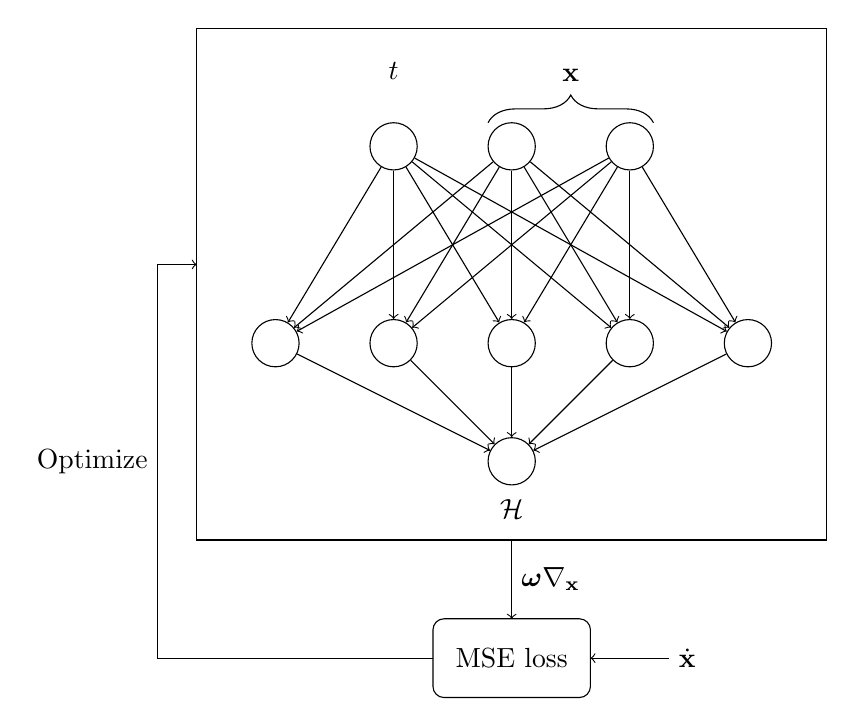
\begin{tikzpicture}
		\tikzstyle{neuron}=[circle,draw=black,minimum size=0.6cm,inner sep=0]
		\foreach \x in {-1,...,1}
			\node[neuron] (input\x) at (1.5*\x, 0) {};
		\foreach \x in {-2,...,2}
			\node[neuron] (hidden\x) at (1.5*\x, -2.5) {};
		\node[neuron] (output) at (0, -4) {};

		\foreach \xin in {-1,...,1}
			\foreach \xout in {-2,...,2}
				\path[->] (input\xin) edge (hidden\xout);
		\foreach \xin in {-2,...,2}
			\path[->] (hidden\xin) edge (output);

		\node at (-1.5,0.6cm+10pt) {$t$};
		\draw[decorate,decoration={brace,amplitude=10pt},xshift=0,yshift=0.6cm]
				(-0.3,-0.3) -- (1.8,-0.3) node[midway,yshift=0.6cm] {$\mathbf x$};
		\node at (0,-4.6) {$\mathcal H$};

		\draw (-4,1.5) rectangle (4,-5);
		\draw[->] (0,-5) -- (0,-6) node[midway,anchor=west] {$\boldsymbol\omega\nabla_{\mathbf x}$};
		\draw[rounded corners] (-1,-6) rectangle (1,-7);
		\node at (0,-6.5) {MSE loss};
		\node[anchor=west] (truth) at (2,-6.5) {$\dot{\mathbf x}$};
		\draw[->] (truth) -- (1,-6.5);

		\draw[->] (-1,-6.5) -- (-4.5,-6.5) -- (-4.5,-1.5) -- (-4,-1.5);
		\node[anchor=east] at (-4.5,-4) {Optimize};
	\end{tikzpicture}
	\caption{The train circle of a supervised hamiltonian neural network \cite{greydanus2019hamiltonian}}
	\label{fig:sup_train}
\end{figure}

\begin{figure}[h!]
	\centering
	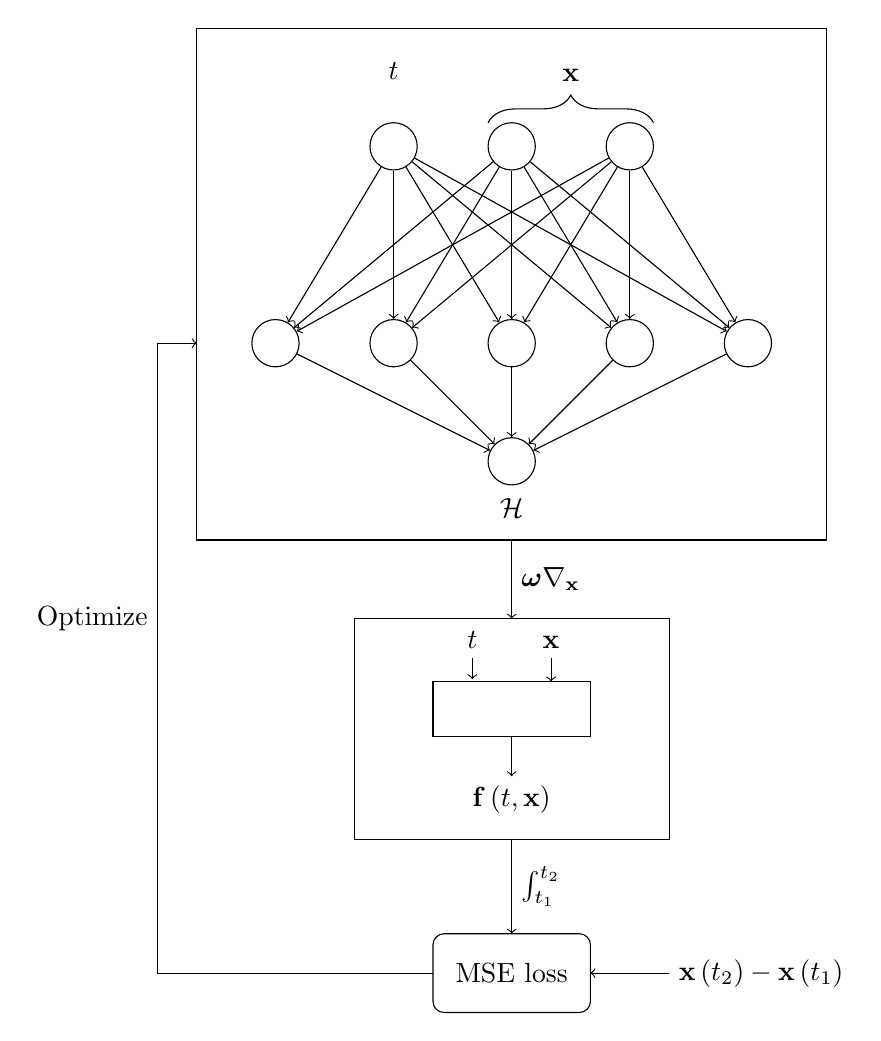
\begin{tikzpicture}
		\tikzstyle{neuron}=[circle,draw=black,minimum size=0.6cm,inner sep=0]
		\foreach \x in {-1,...,1}
			\node[neuron] (input\x) at (1.5*\x, 0) {};
		\foreach \x in {-2,...,2}
			\node[neuron] (hidden\x) at (1.5*\x, -2.5) {};
		\node[neuron] (output) at (0, -4) {};

		\foreach \xin in {-1,...,1}
			\foreach \xout in {-2,...,2}
				\path[->] (input\xin) edge (hidden\xout);
		\foreach \xin in {-2,...,2}
			\path[->] (hidden\xin) edge (output);

		\node at (-1.5,0.6cm+10pt) {$t$};
		\draw[decorate,decoration={brace,amplitude=10pt},xshift=0,yshift=0.6cm]
				(-0.3,-0.3) -- (1.8,-0.3) node[midway,yshift=0.6cm] {$\mathbf x$};
		\node at (0,-4.6) {$\mathcal H$};

		\draw (-4,1.5) rectangle (4,-5);
		\draw[->] (0,-5) -- (0,-6) node[midway,anchor=west] {$\boldsymbol\omega\nabla_{\mathbf x}$};

		\draw (-2,-6) rectangle (2,-8.8);
		\node[anchor=south] (tin) at (-0.5,-6.5) {$t$};
		\node[anchor=south] (xin) at (0.5,-6.5) {$\mathbf x$};
		\draw[->] (tin) -- +(0,-0.5);
		\draw[->] (xin) -- +(0,-0.5);
		\draw (-1,-6.8) rectangle (1,-7.5);
		\node[anchor=north] (fout) at (0,-8) {$\mathbf f\left(t,\mathbf x\right)$};
		\draw[->] (0,-7.5) -- (fout);

		\draw[->] (0,-8.8) -- (0,-10) node[midway,anchor=west] {$\int_{t_1}^{t_2}$};
		\draw[rounded corners] (-1,-10) rectangle (1,-11);
		\node at (0,-10.5) {MSE loss};
		\node[anchor=west] (truth) at (2,-10.5) {$\mathbf x\left(t_2\right)-\mathbf x\left(t_1\right)$};
		\draw[->] (truth) -- (1,-10.5);

		\draw[->] (-1,-10.5) -- (-4.5,-10.5) -- (-4.5,-2.5) -- (-4,-2.5);
		\node[anchor=east] at (-4.5,-6) {Optimize};
	\end{tikzpicture}
	\caption{The train circle of a self-supervised hamiltonian neural network}
	\label{fig:selfsup_train}
\end{figure}

\section{The training}

Our goal is to derive the function $\left(t,\mathbf x\right)\mapsto\mathcal H$
according to the dataset containing a series of samples in form of $\left(t,\mathbf x\right)$ on a series of possible motions of the system.

The dataset does not contain the $\dot{\mathbf x}$ infomation,
which acts as the ground truth in the supervised model \cite{greydanus2019hamiltonian}.
Our model is self-supervised, and thus does not need the $\dot{\mathbf x}$ infomation.

The model uses the loss inspired from Equation \ref{eq:int}
\begin{equation}
	\mathcal L:=\operatorname{MSE}\left(\mathbf x\left(t_1\right)+\int_{t_1}^{t_2}\boldsymbol\omega\nabla_{\mathbf x}\mathcal H\mathrm dt,\mathbf x\left(t_2\right)\right),
\end{equation}
where $\left(t_1,\mathbf x\left(t_1\right)\right)$ and $\left(t_1,\mathbf x\left(t_1\right)\right)$
are 2 samples from the same motion of the system.
The complete process of a traning circle is shown in Figure \ref{fig:selfsup_train}.
For comparison, the train circle of the supervised hamiltonian neural network
is shown in Figure \ref{fig:sup_train}.

The Adam optimizer \cite{kingma2017adam} is used for optimizing the neural network.

\section{Tasks}

\subsection{Free particle}

A free particle is a system with 1 DOF whose hamiltonian is
\begin{equation*}
	\mathcal H\left(t,q,p\right):=\frac{p^2}{2m},
\end{equation*}
where $m$ is the mass of the particle.
To be simple, we take $m=1/2$.

\subsection{Harmonic oscillator}

\bibliographystyle{abbrv}
\bibliography{selfsup_hnn}

\end{document}
